\documentclass[11pt]{article}
\usepackage[utf8]{inputenc}
\usepackage{amsmath}
\usepackage{amsfonts}
\usepackage{graphicx}
\usepackage{booktabs}
\usepackage{hyperref}
\usepackage{natbib}
\usepackage{geometry}
\usepackage{float}
\geometry{a4paper, margin=1in}\usepackage{setspace}
\singlespacing

\title{Computational Approaches to Nim: Verifying the Sprague-Grundy Theorem and Training Neural Networks}

\author{
Minghan Wu\thanks{St. Mildred's-Lightbourn School}
}



\date{August 2026}

\begin{document}

\maketitle

\begin{abstract}
Nim is a classical two-player combinatorial game. The Sprague-Grundy Theorem states that any finite impartial normal-play game is equivalent to a Nim pile of a specific size. By calculating the XOR sum at the current state, we are able to determine if a position is a winning position and play optimally. We found relatively little work that tests the theorem computationally or uses finite cases to explore ordinal variants. In this paper, we verify the theorem computationally: a recursive simulator based on the mex (minimum excluded value) definition predicts the winner of all 10,000 randomly generated games correctly. We then approximate ordinal piles with finite surrogates and find that game length grows linearly in the approximation size. Finally, we train a multi-layer perceptron to predict optimal moves from pile sizes alone; it reaches 89.77\% accuracy without being given the XOR rule. This suggests that the network learned part of the strategy, although its accuracy was not high enough to show that it learned the exact XOR rule. Code available at \href{https://github.com/Minghan-Wu/Nim-simulator}{GitHub}.
\end{abstract}

\section{Introduction}
Combinatorial games are two-player games of perfect information in which players alternate turns. Combinatorial games are deterministic, meaning that the final outcome can be determined by game states and under normal play, each finite position is either winning or losing for the player to move. Combinatorial game theory began in 1901 when Charles L.Bouton solved the game of Nim~\cite{bouton1901nim}. In the 1930s, the creation of the Sprague-Grundy Theorem by Roland Sprague and Patrick Grundy proved that every finite impartial normal-play game is equivalent to a single pile of Nim~\cite{sprague1935, grundy1939}. 

Nim was the subject of some of the earliest dedicated computing devices, including the electro-mechanical Nimatron developed in 1940~\cite{condon1940nimatron} and the digital Nimrod computer exhibited in 1951~\cite{norman1951nimrod}. However, as game states scale today, the computational cost of resolving game lengths diverges significantly.

A related question has attracted attention more recently: can a standard neural network learn the bitwise-XOR structure behind the Sprague-Grundy Theorem from examples alone, without the rule being programmed in~\cite{shalev2017failures, riis2024mastering}? 

This paper combines the two perspectives. We build a recursive simulator based on the minimum excluded value and use it to verify finite Nim positions, apply it to finite approximations of ordinal Nim, and train a multi-layer perceptron (MLP) to predict winning moves directly from pile sizes.


\section{Background}
\subsection{Nim and Special Cases}
% Your PPT notes here
In the game Nim, two players take turns removing stones from multiple piles, each pile with a non-zero number of stones. Whoever takes the last stone wins. Since both players can see the current state and observe all moves, Nim is a finite, deterministic game of perfect information. By the Fundamental Theorem of Finite Games, there exists a winning strategy for either the first or second player. 

We now show that several special cases have simple winning strategies. 
\begin{itemize}
    \item \textbf{1 stone per pile}: Even number of piles $\xrightarrow{}$ second player wins; Odd number of piles $\xrightarrow{}$ first player wins. 
    \item \textbf{Two identical piles $(n,n)$}: Second player always wins by mirroring the first player's moves. 
    \item \textbf{Two unequal piles $(n,m)$ with $n>m$}: First player wins by turning the game to $(m,m)$, then mirroring what the second player does. 
\end{itemize}

The general winning strategy uses the XOR sum of all pile sizes, described by the Sprague-Grundy Theorem below. 

\subsection{Sprague-Grundy Theorem}
% MEX definition, XOR shortcut
The Sprague-Grundy Theorem applies to every impartial two-player game, in which the available moves and the winning or losing only depends on the current game state~\cite{cpalgorithms2024nim}. Each game state has a Grundy number. A state with no available moves has Grundy number 0; every other state's Grundy number is the mex of the Grundy numbers of the states reachable from it, where mex(S) denotes the smallest non-negative integer not in S. For example, $\text{mex}(\{0,1,3\})=2$. The Grundy value $g(S)$ of a game state $S$ can be recursively defined as:

\[
g(S) = \text{mex}\left(\{g(S') : S \to S'\}\right)
\]

For a single pile of size $n$ in Nim, the Grundy number is $n$, since there exist possible moves that can lead to piles of size $0, 1, \dots, n-1$, and $\text{mex}(\{0,1,\dots,n-1\}) = n$.

The Sprague-Grundy Theorem states that for a disjunctive sum of Nim piles, the Grundy value is the \textbf{XOR sum} of the individual pile sizes:

\[
g(p_1, p_2, \dots, p_k) = p_1 \oplus p_2 \oplus \dots \oplus p_k
\]

where $\oplus$ is the bitwise XOR. For example, $5 \oplus 7\oplus9=11$.

The winning condition follows directly: If the XOR sum is non-zero, the first player has a winning strategy by turning the XOR sum to zero; if the XOR sum is zero, then the second player has a winning strategy. 





\section{Methods}
This section describes the framework used to verify the Sprague-Grundy Theorem, explore and approximate ordinal cases, and evaluate whether a simple neural network can learn optimal Nim play from examples. 
\subsection{Recursive Nim Simulator}
% Recursive MEX code explanation
First, a recursive Nim simulator was implemented by the definition of Grundy values. The game state is represented as a tuple of pile sizes. An empty pile is considered to have a game value of 0. Since the order of piles does not matter, each state was canonicalized by sorting its pile sizes, so (5,2) and (2,5) are treated as the same state. Memoization stored each previously computed Grundy value in a dictionary keyed by the canonical tuple. 

During the game, each move is generated by selecting one non-empty pile and removing a number between one and all stones from that pile. This approach directly implements the recursive definition of Sprague-Grundy Theorem instead of using the XOR shortcut, which allows us to verify the theorem computationally. As a sanity check, the simulator's Grundy values matched the XOR sums on small examples such as (3,3), (5,3), and (5,7,9).

\subsection{Finite Case Verification}
For the finite case, we generated random Nim positions with maximum five piles, each pile containing at most 20 stones. For each position, we calculated the Grundy value defined by the recursive simulator, then simulated the game, and compared the predicted winner with the actual winner with both sides playing optimally. 

\subsection{Ordinal Approximation}
\label{sec: ordinal rules}
% ω ≈ N strategy
%To approximate cases when the number of stones in each pile is approaching infinity, we replaced ordinals, which are not able to be computed, with increasing large values. Specifically, we represented $\omega$ as $N$ and used expressions such as $3N+2$ and $N+1$ to represent $3\omega+2$ and $\omega+1$, respectively. We then simulated each game withe the XOR shortcut to reduce runtime. The purpose of this experiment is to study how game length changes as the size of piles increases. 

Our ordinal experiments consider the family of finite Nim positions $(3N+2, N+1)$ for increasing positive integers $N$ to approximate $(3\omega+2, \omega+1)$. We evaluated this family of positions using an efficient bitwise XOR simulation engine. 

To resolve the game deterministically, we define a two-part rule for each move:
\begin{enumerate}
    \item When in a winning state ($\text{Nim-sum} \neq 0$), the player executes the unique optimal move that reduces the Nim-sum to zero.
    \item When in a losing state ($\text{Nim-sum}=0$), where no winning move exists, the player defaults to a minimal delay strategy by removing exactly one stone from the first available non-empty pile. 
\end{enumerate}

\subsection{Neural Network Architecture}
% MLP details
We framed optimal move selection as a 5-class classification task to test whether a feedforward network can learn winning strategies from state representations alone. Each input sample was a 5-dimensional vector representing pile sizes, zero-padded for configurations with fewer than five piles. 

The target label corresponds to the index of the pile ($i \in \{0,1,2,3,4\}$) from which stones must be removed to transition the board to a state with a Grundy value of 0. When multiple piles admitted a valid winning transition, the ground truth was assigned to the first valid pile index encountered during linear search. Losing initial positions ($\text{Nim-sum}=0$) were excluded from training since no winning transition exists.

We used a multi-layer perceptron (MLP) with two hidden layers containing 64 and 32 neurons, respectively, with ReLU activation functions and standard cross-entropy loss.

\subsection{Implementation Details}
All experiments were implemented in Python on Google Colab notebook. The recursive simulator used memoization to reduce cases, and the neural network experiment was run on a standard CPU. Results were recorded through repeated simulation and summarized using tables and plots for inclusion in the paper.

\section{Experiments}
We conducted three primary experiments to evaluate our computational models: verifying the Sprague-Grundy Theorem on finite games, simulating ordinal approximations, and assessing the neural network's ability to learn optimal Nim strategy. 
\subsection{Finite Verification}
We verified our recursive mex simulator by simulating 10,000 randomly generated Nim games. Each game consisted of one to five piles with sizes uniformly distributed between 1 and 20 stones. 

Over the 10,000 simulated games, the average game length was 8.24 moves. The simulator recorded Player 1 winning 9703 times (starting states where the Grundy value was non-zero) and Player 2 winning 297 times (starting states where the Grundy value was zero). This imbalance is expected: a random position is far more likely to have a non-zero XOR sum than one of exactly zero.

In every instance, the simulator's prediction matched the theorem's (100.00\% accuracy), confirming that the implementation agrees with Sprague-Grundy theory over the tested range.

\subsection{Ordinal Divergence}
% Include your plot!
%For ordinal approximation, we replaced the ordinal Nim configuration ($3\omega+2$, $\omega+1$) with ($3N+2$, $N+1$) for $N \in \{100, 500, 1000, 5000, 10000, 50000\}$.

%The results shown in Figure~\ref{fig:ordinal} demonstrates a strict linear divergence. The game length increases unboundedly to $N$. This behavior illustrates the property of transfinite ordinal games: as the game approaches an infinite state, the number of required moves scales infinitely. 

For each $N \in \{100, 500, 1000, 5000, 10000, 50000\}$, we simulated the finite state $(3N+2, N+1)$ under the rules described in Section~\ref{sec: ordinal rules}. As shown in Figure~\ref{fig:ordinal}, the observed game length was $2N+3$. Thus, the runtime of this simulation increases linearly with $N$. 
\begin{figure}[H]
\centering
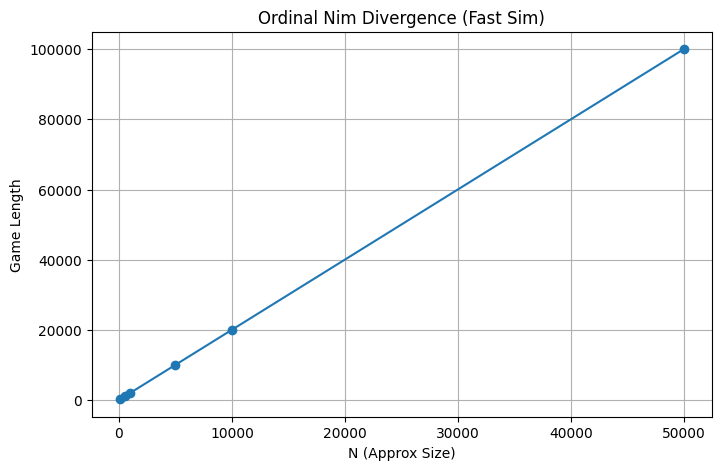
\includegraphics[width=0.8\textwidth]{Ordinal_Nim_Divergence.png}
\caption{Game length divergence in ordinal Nim approximation.}
\label{fig:ordinal}
\end{figure}

\subsection{Neural Network Results}
From our initial generation of 10,000 training and 2000 testing examples, discarding losing positions (where no optimal move exists) resulted in a final dataset of 9457 training positions and 1897 testing positions. 

The MLP reached 89.77\% accuracy, well above random guessing, and the training loss (Figure~\ref{fig:nn}) converged quickly. The network therefore picked up much of the winning strategy from raw pile sizes alone, without being given the XOR rule.

\begin{figure}[H]
\centering
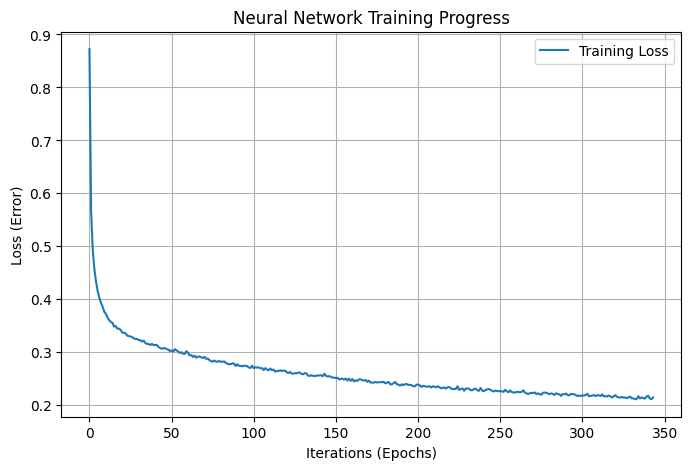
\includegraphics[width=0.8\textwidth]{Lost_Curve.png}
\caption{Neural network training loss.}
\label{fig:nn}
\end{figure}

\section{Discussion and Conclusion}
The results of our experiments demonstrate the efficiency of using algorithmic evaluation to verify classical combinatorial game theory. Our finite game simulator verified the Sprague-Grundy Theorem with 100\% accuracy across 10000 randomized states. Our ordinal approximations showed a strict linear divergence. 

The MLP's 89.77\% accuracy is notable given that XOR-type functions are known to be hard for gradient-based learning~\cite{shalev2017failures}, but it falls short of 100\%, so we cannot conclude that the network learned the exact bitwise rule.

Future work could test other ordinal families and architectures such as Transformers, which may come closer to exact generalization.

\section*{Acknowledgements}
The author used an AI assistant (Perplexity) to support drafting, editing, and organization of portions of the manuscript text, including sections of the introduction, discussion, and conclusion. All research design, experiments, code, numerical results, and analysis were independently developed and verified by the author.


\bibliographystyle{plain}
\bibliography{main}


\end{document}
